\documentclass[man,floatsintext,12pt]{apa7}

\usepackage[american]{babel}
\usepackage{csquotes}
\usepackage[style=apa,sortcites=true,sorting=nyt,backend=biber]{biblatex}
\DeclareLanguageMapping{american}{american-apa}
\addbibresource{references.bib}

\usepackage{graphicx}
\usepackage{booktabs}
\usepackage{siunitx}
\usepackage{amsmath}

\title{respyra: A General-Purpose Respiratory Tracking Toolbox for Interoception Research}
\shorttitle{Respiratory Tracking Toolbox}

\authorsnames{Micah Allen}
\authorsaffiliations{Aarhus University}

\abstract{Respiratory interoception is increasingly recognized as a key modality linking bodily sensation to emotional experience and self-regulation. However, few tools exist for studying the sensorimotor dynamics of voluntary breathing control. Here we present \textit{respyra}, an open-source Python toolbox that integrates a Vernier Go Direct Respiration Belt with PsychoPy to enable real-time respiratory tracking experiments. Participants follow a sinusoidal target with their breathing while receiving continuous visual biofeedback. The toolbox supports configurable experimental conditions including multi-frequency target waveforms and visuomotor perturbations (visual gain manipulation), in which the displayed breathing trace is amplified or attenuated relative to ground truth. The visuomotor perturbation is designed to dissociate two components of respiratory control: veridical feedback conditions measure baseline respiratory tracking ability, while perturbed conditions probe the capacity to remap sensorimotor relationships when visual feedback is altered. We report a single-participant validation study comprising 48 trials across four sessions under veridical and $2\times$ gain perturbation conditions in a blocked, counterbalanced design. The participant achieved accurate respiratory tracking under veridical feedback (visual MAE = \SI{0.243}{\newton}) with substantially increased error under perturbation (visual MAE = \SI{0.538}{\newton}; perturbation ratio = $2.2\times$). Perturbed trials showed within-block adaptation that degraded across sessions, while veridical performance remained stable---suggesting that fatigue selectively impairs sensorimotor remapping rather than basic respiratory control. Split-half reliability was good (Spearman--Brown = .86). The toolbox is freely available and designed to facilitate research on respiratory sensorimotor control, interoceptive learning, and breathing-based interventions.}

\keywords{respiratory interoception, sensorimotor adaptation, breathing, visuomotor perturbation, psychophysics, open-source toolbox}

\begin{document}
\maketitle

\section{Introduction}

Interoception---the sensing, interpretation, and integration of signals originating from within the body---is increasingly recognized as a fundamental mechanism underlying emotional experience, cognitive function, and behavioral self-regulation \parencite{garfinkel2015knowing, suksasilp2022towards}. Contemporary research distinguishes between interoceptive accuracy (objective behavioral performance), interoceptive sensibility (self-reported beliefs), and interoceptive awareness (metacognitive correspondence between accuracy and confidence), revealing that these dimensions are largely modality-specific \parencite{garfinkel2015knowing, banellis2026interoceptive}.

While the cardiac axis has dominated interoception research, respiratory interoception---or respiroception---offers a uniquely important physiological modality because it is closely linked to affect and, critically, is amenable to direct conscious control \parencite{nikolova2022respiratory, harrison2021interoception}. Slow deep breathing at approximately 0.1~Hz stimulates arterial baroreceptors, enhances respiratory sinus arrhythmia, and reduces sympathetic output \parencite{gholamrezaei2021psychophysiological}. Beyond autonomic regulation, paced slow breathing reduces anticipatory anxiety and suppresses cortical beta-band arousal markers \parencite{luo2025effect}. The respiratory cycle itself modulates neural oscillations and differentially gates exteroceptive versus interoceptive processing across inhalation and exhalation phases \parencite{molle2022respiratory}.

Measuring respiroception has relied primarily on detection paradigms, such as the Filter Detection Task \parencite{harrison2021interoception} and the Respiratory Resistance Sensitivity Task \parencite{nikolova2022respiratory}, which quantify perceptual sensitivity to inspiratory loads. However, these approaches focus on interoceptive detection rather than on the sensorimotor dynamics of voluntary breathing control---that is, the ability to precisely modulate one's own respiratory output to match a prescribed target. This motor control dimension of breathing is central to breathing-based interventions and meditation practices, yet it has received comparatively little experimental attention.

The study of sensorimotor control offers well-established paradigms for investigating how the motor system adapts to perturbations in visual feedback. In visuomotor reaching studies, participants learn to compensate for rotated or scaled cursor feedback, revealing the dynamics of sensorimotor adaptation, error correction, and internal model updating \parencite[e.g.,][]{krakauer2019motor}. Importantly, veridical and perturbed feedback conditions probe dissociable constructs: veridical tracking reflects baseline motor control ability, while perturbed tracking additionally engages the capacity to remap sensorimotor relationships when feedback is altered. The ratio of perturbed to veridical error isolates this remapping cost independent of baseline ability, offering a promising individual-differences metric for future group studies. Applying analogous perturbation paradigms to respiratory control could illuminate how individuals monitor and correct their breathing output, with implications for understanding both healthy respiratory regulation and clinical conditions involving dysfunctional breathing patterns.

Here we present \textit{respyra}, an open-source Python toolbox for conducting respiratory tracking experiments with real-time biofeedback and visuomotor perturbation capabilities (Figure~\ref{fig:schematic}). The toolbox integrates a commercially available respiration belt with PsychoPy for stimulus-precise experiment control. We describe the system architecture and experimental protocol, and report a single-participant validation study (48 trials across four sessions) demonstrating that (a) participants can accurately track sinusoidal breathing targets under veridical feedback, (b) visual gain perturbations reliably increase tracking error, (c) perturbed trials show within-block adaptation that degrades with fatigue while veridical performance remains stable, and (d) the task produces reliable trial-level measurements.

\section{Method}

\begin{figure}[ht]
\centering
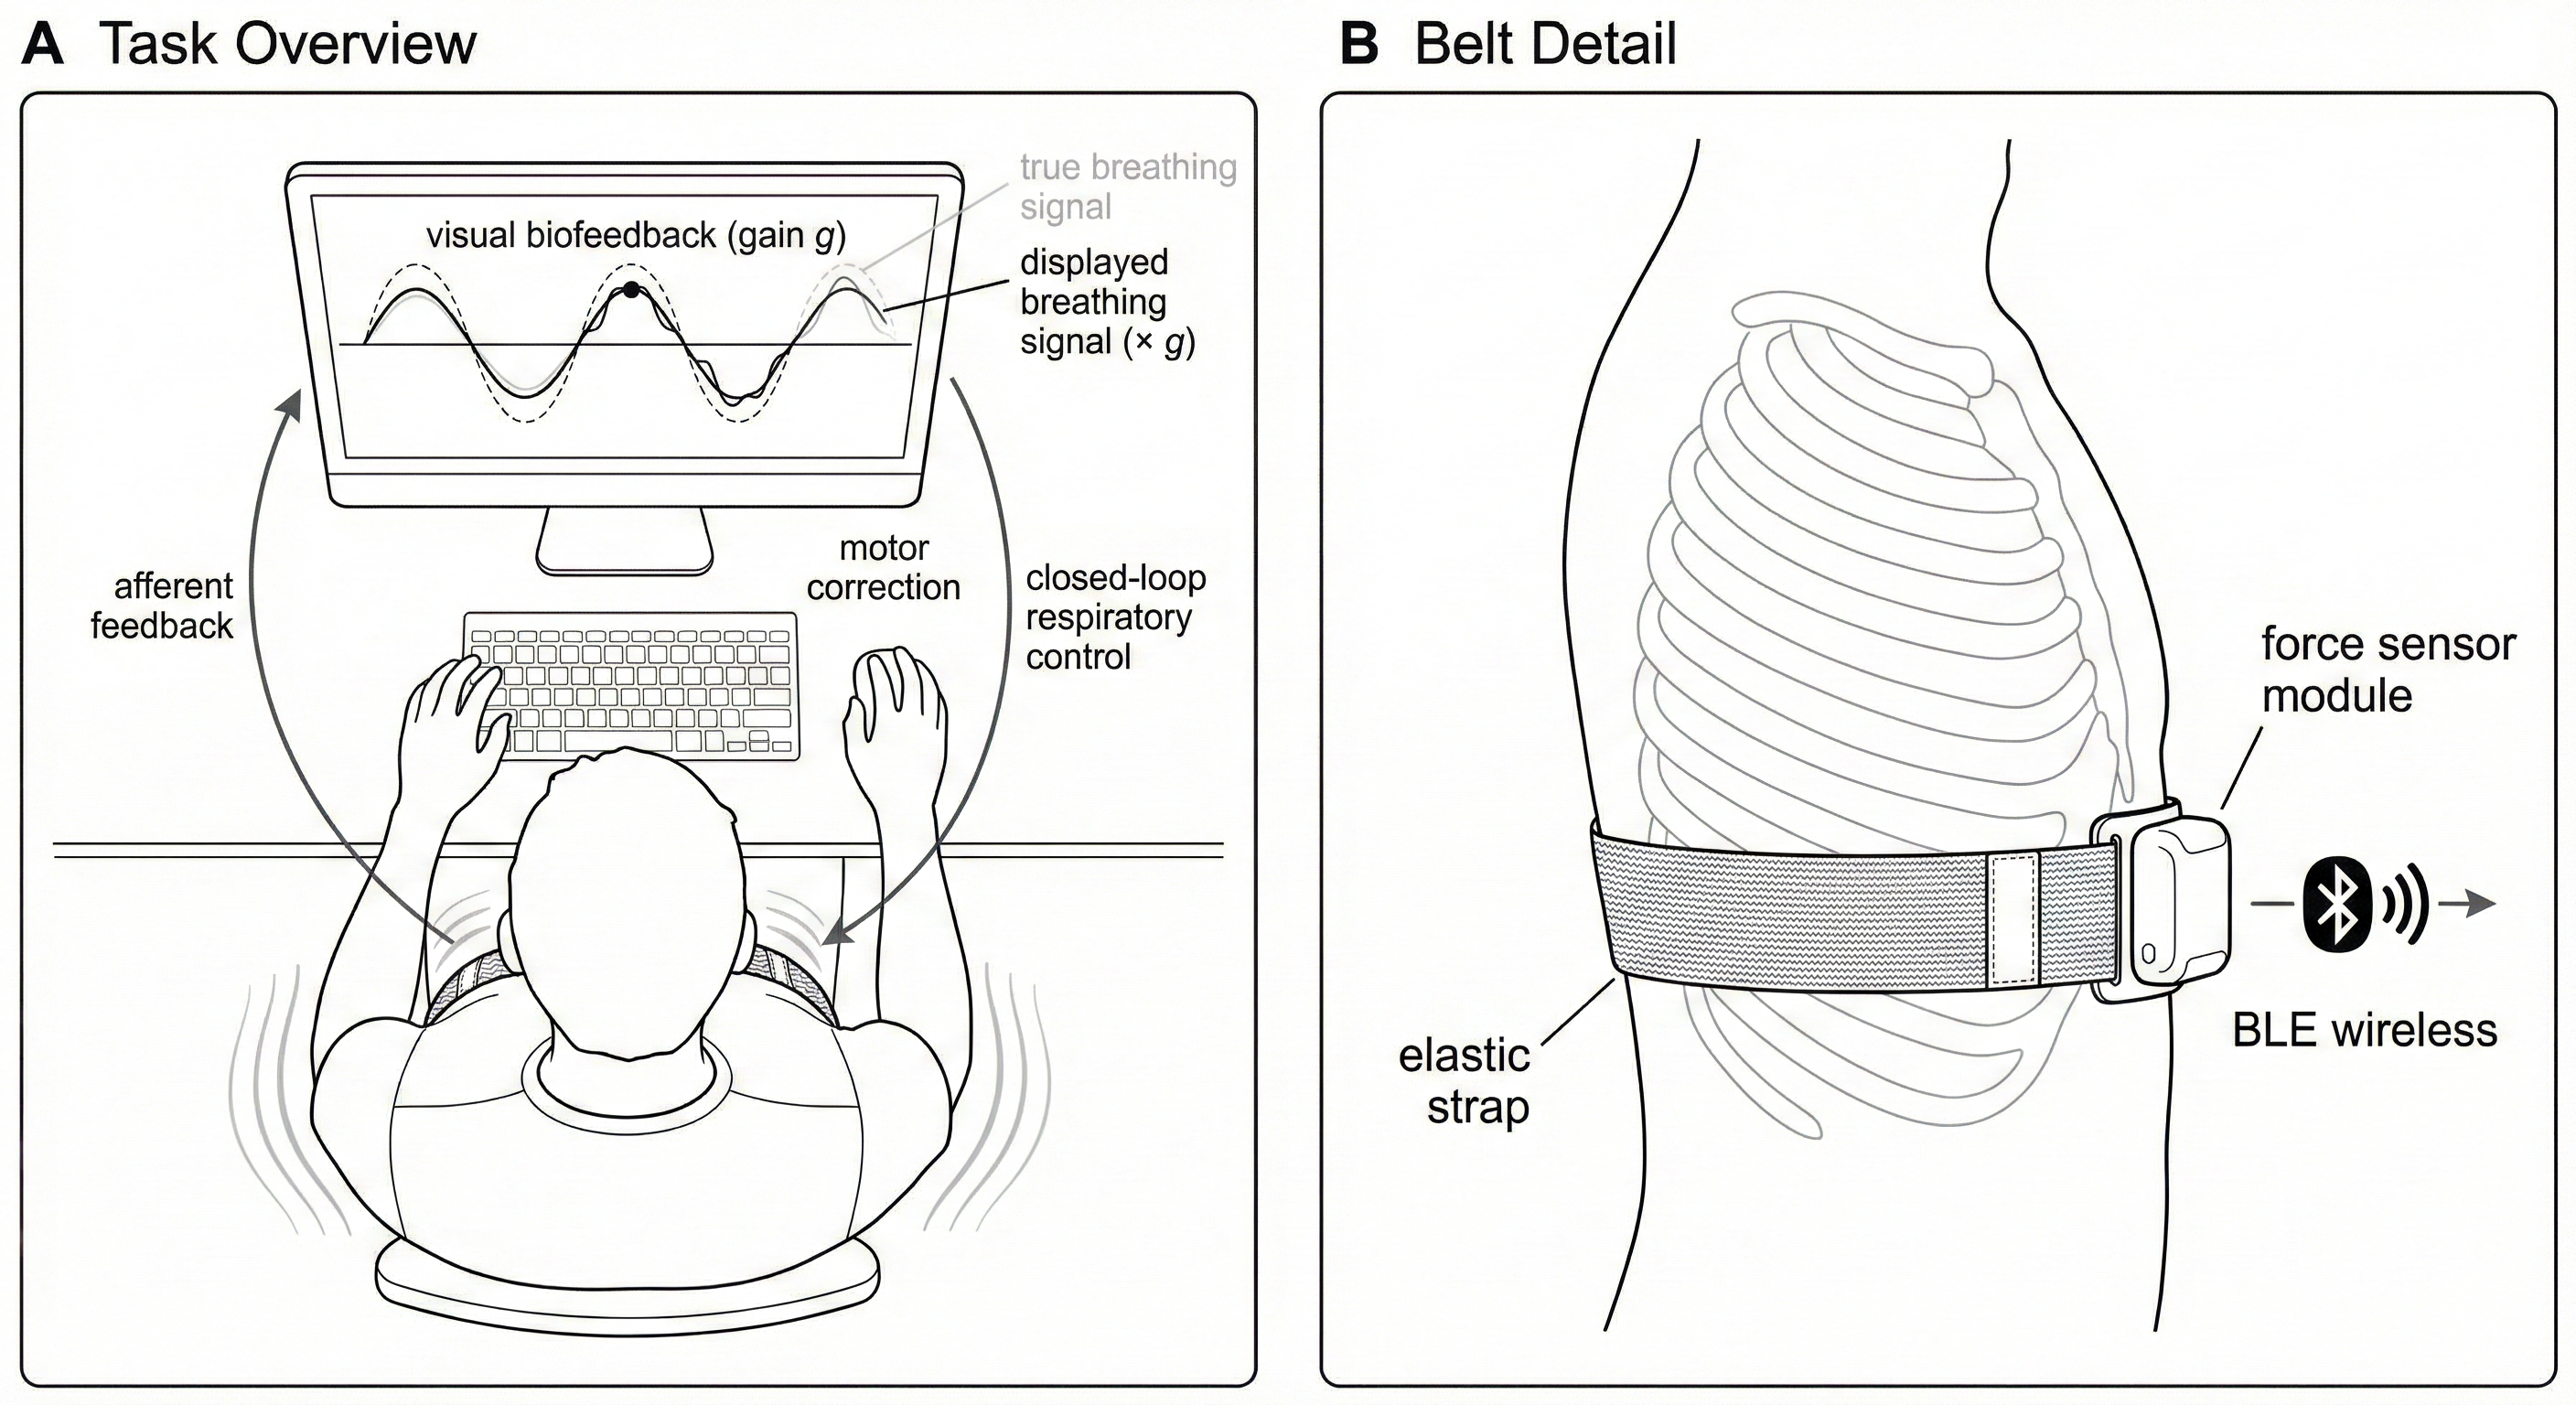
\includegraphics[width=\textwidth]{fig_task_schematic.png}
\caption{Schematic of the respiromotor tracking task. \textbf{(A)}~Task overview: the participant wears a respiration belt and views a monitor displaying their breathing trace in real time. A sinusoidal target guides the desired breathing pattern. Visual biofeedback can be veridically displayed or scaled by a gain factor $g$, creating a closed-loop sensorimotor control paradigm with afferent feedback and motor correction. \textbf{(B)}~Belt detail: the Vernier Go Direct Respiration Belt (GDX-RB) consists of an elastic strap with an embedded force sensor module that transmits data wirelessly via Bluetooth Low Energy (BLE).}
\label{fig:schematic}
\end{figure}

\subsection{Toolbox Architecture}

\textit{respyra} is implemented in Python 3.10 and integrates two primary components: the Vernier Go Direct Respiration Belt (GDX-RB; Vernier Software \& Technology) for real-time force-based respiratory measurement, and PsychoPy \parencite{peirce2019psychopy} for stimulus presentation and experiment control. The GDX-RB was selected because it is inexpensive, well-documented, available worldwide through educational science suppliers, and offers wireless (BLE) operation out of the box---making it accessible to researchers and teaching laboratories without specialized biomedical equipment budgets. The toolbox is organized into reusable core modules, configuration files, and experiment scripts, following a separation-of-concerns architecture (see Table~\ref{tab:modules}).

\begin{table}[ht]
\caption{Core Modules of the respyra Toolbox}
\label{tab:modules}
\begin{tabular}{lp{10cm}}
\toprule
Module & Description \\
\midrule
\texttt{breath\_belt} & Non-blocking interface to the Vernier GDX-RB. A background thread continuously reads force samples (10~Hz) into a thread-safe queue, allowing the main PsychoPy frame loop to drain samples without blocking. Supports BLE and USB connections. \\
\texttt{display} & PsychoPy window management and a \texttt{SignalTrace} class that renders a scrolling waveform by updating \texttt{ShapeStim} vertices each frame. \\
\texttt{target\_generator} & Generates sinusoidal breathing targets from composable frequency--cycle segment definitions. Supports multi-segment waveforms with phase-continuous boundaries. \\
\texttt{data\_logger} & Incremental CSV logging with per-row flush for crash resilience. \\
\texttt{events} & Keyboard input helpers wrapping PsychoPy's event module. \\
\bottomrule
\end{tabular}
\end{table}

The respiration belt measures chest expansion force in Newtons (0--50~N range) via a force sensor embedded in an elastic chest strap. The belt communicates with the host computer via Bluetooth Low Energy (BLE) or USB. To resolve a platform-specific conflict on Windows---where PsychoPy's graphics backend initializes COM in single-threaded apartment (STA) mode while the BLE scanner requires multi-threaded apartment (MTA) mode---the toolbox connects the belt \textit{before} importing PsychoPy modules.

Experimental conditions are defined using a \texttt{ConditionDef} dataclass specifying a name, a list of \texttt{SegmentDef} objects (each with a target frequency in Hz and an integer cycle count), and an optional \texttt{feedback\_gain} parameter. The use of integer cycle counts ensures phase continuity at segment boundaries, allowing seamless composition of multi-frequency waveforms.

\subsection{Visual Feedback and Perturbation}

The task display consists of two visual elements: a scrolling waveform trace showing the participant's real-time breathing signal, and a target dot that traverses a sinusoidal path at the prescribed target frequency. The dot's vertical position indicates the target force, and its color provides continuous error feedback using an HSV color mapping from green (low error) through yellow to red (high error), with a square-root transfer function for perceptual salience.

The visuomotor perturbation is implemented as a multiplicative gain applied to the visual trace display:
\begin{equation}
f_{\text{display}} = c + g \cdot (f_{\text{actual}} - c)
\label{eq:gain}
\end{equation}
where $f_{\text{actual}}$ is the raw belt force, $c$ is the participant's breathing center (from calibration), and $g$ is the feedback gain. When $g = 1.0$, the display is veridical. When $g > 1.0$, displayed deviations from center are amplified, requiring the participant to breathe with \textit{smaller} amplitude to match the visual target. The target dot position remains anchored to the physical target waveform, while the dot's color feedback reflects the \textit{visual error}---the discrepancy between the target and the displayed trace (see Equation~\ref{eq:visual_error})---ensuring that color feedback is consistent with the participant's visual experience of their tracking performance.

\subsection{Calibration}

Prior to the experimental trials, participants complete a 15-second range calibration phase during which they take several comfortable deep breaths. The force data collected during this phase are used to establish the participant's achievable breathing range. To ensure robust calibration, the toolbox applies percentile-based outlier rejection (5th--95th percentile clipping), excluding extreme values caused by movement artifacts or sensor saturation. If force values approach the sensor limits ($\leq$~\SI{0}{\newton} or $\geq$~\SI{40}{\newton}), a warning dialog alerts the experimenter that the belt may be too tight. The clipped range is then scaled by a configurable factor (default 0.80) to set the target waveform amplitude, ensuring the sinusoidal target stays within the participant's comfortable range.

\subsection{Experimental Protocol}

Each session consists of a range calibration phase followed by a series of tracking trials. Each trial comprises three phases:

\begin{enumerate}
\item \textbf{Baseline} (10~s): The participant breathes naturally. Force data from this phase are used to compute a trial-specific breathing center via the midpoint of the observed range.
\item \textbf{Countdown} (3~s): A ``3\ldots2\ldots1'' countdown during which the target dot smoothly blends from the participant's current respiratory position into the target waveform trajectory, providing a gradual transition into tracking.
\item \textbf{Tracking}: The participant follows the sinusoidal target dot with their breathing for a duration determined by the trial's frequency--cycle segment definitions. Force, target, and signed error are logged at every sample (\textasciitilde10~Hz). At the conclusion of each trial, mean absolute tracking error is displayed as performance feedback.
\end{enumerate}

Trial conditions are managed using PsychoPy's \texttt{TrialHandler}, supporting both blocked and randomized presentation orders across configurable numbers of repetitions.

\subsection{Validation Data Collection}

To validate the toolbox, a single experienced participant (male, first author) completed four sessions in a single sitting. Each session consisted of 12 tracking trials: six veridical feedback trials ($g = 1.0$) and six perturbed feedback trials ($g = 2.0$), presented in a blocked design. Each trial comprised four sinusoidal cycles at 0.1~Hz (40~s tracking duration). The starting condition was counterbalanced across sessions: sessions 1 and 3 began with the veridical block, while sessions 2 and 4 began with the perturbed block. Between sessions, the participant had the option to recalibrate the belt. The belt was worn around the lower ribcage and connected via BLE at 10~Hz sampling. The display was presented on a 1920$\times$1080 monitor at 57~cm viewing distance.

\subsection{Data Analysis}

Tracking performance was quantified using visual mean absolute error (visual MAE)---defined as the mean absolute deviation between the target waveform and the displayed feedback trace during each trial's tracking phase:
\begin{equation}
\text{Visual MAE} = \frac{1}{n} \sum_{i=1}^{n} \left| f_{\text{target},i} - f_{\text{display},i} \right|
\label{eq:visual_error}
\end{equation}
where $f_{\text{display}}$ is defined by Equation~\ref{eq:gain}. For veridical trials ($g = 1$), visual MAE equals the physical tracking error. For perturbed trials ($g > 1$), visual MAE captures the error as experienced by the participant in the displayed feedback---the quantity the participant actively optimizes in the closed-loop control task.

The \textit{perturbation ratio} was computed as the ratio of perturbed visual MAE to veridical visual MAE within each session, providing a normalized index of the cost of sensorimotor remapping independent of baseline tracking ability.

The ratio of root mean square error to MAE (RMSE/MAE ratio) was computed as a secondary metric of error distribution shape. For normally distributed errors, this ratio equals $\sqrt{\pi/2} \approx 1.253$; values exceeding this reference indicate heavy-tailed error distributions with intermittent large deviations, suggestive of attentional lapses or control instability.

Respiratory metrics---breaths per minute (BPM) and peak-to-trough breathing depth---were computed for each trial using SciPy peak detection on the force signal. Breath phase was labeled continuously based on the gradient of the target sinusoid (rising phase = inspiration, falling phase = expiration).

Split-half reliability was assessed by correlating visual MAE between odd-numbered and even-numbered trials within each condition, with the Spearman--Brown prophecy formula applied to estimate full-test reliability.

All analyses were conducted at the trial level (each trial = one observation, $N = 48$). Statistics were computed using Python with pandas, NumPy, and SciPy.

\section{Results}

\subsection{Calibration}

Prior to each session, the participant completed the range calibration procedure. Calibration amplitude varied across sessions, with Session~1 producing a notably large target amplitude due to an excessively deep calibration breath, which increased the difficulty of tracking---particularly under perturbed feedback where the required breathing amplitude was halved by the $2\times$ gain. Baseline breathing centers were stable within sessions, indicating consistent resting breathing position.

\subsection{Tracking Performance}

\begin{table}[ht]
\centering
\caption{Session-level descriptive statistics for the single-participant validation study (4~sessions, 12~trials each). BPM = breaths per minute; Depth = peak-to-trough breathing amplitude. MAE values are visual MAE (mean absolute error between target and displayed feedback; for veridical trials, visual MAE equals physical MAE). Dur.\ = session duration in minutes. Values are $M \pm SD$ across trials.}
\label{tab:session_stats}
\small
\begin{tabular}{c c r r@{\,}l r@{\,}l r r@{\,}l r@{\,}l}
\toprule
Session & $N$ & Dur. & \multicolumn{2}{c}{BPM} & \multicolumn{2}{c}{Depth (N)} & Cycles & \multicolumn{2}{c}{Verid.\ MAE (N)} & \multicolumn{2}{c}{Pert.\ MAE (N)} \\
\midrule
  1 & 12 & 10.8 & 6.0 & $\pm$ 0.22 & 5.80 & $\pm$ 1.35 & 37 & 0.321 & $\pm$ 0.058 & 0.837 & $\pm$ 0.289 \\
  2 & 12 & 10.8 & 6.1 & $\pm$ 0.21 & 2.46 & $\pm$ 0.64 & 37 & 0.154 & $\pm$ 0.023 & 0.259 & $\pm$ 0.023 \\
  3 & 12 & 10.8 & 6.0 & $\pm$ 0.21 & 3.64 & $\pm$ 0.95 & 37 & 0.230 & $\pm$ 0.018 & 0.411 & $\pm$ 0.100 \\
  4 & 12 & 10.8 & 6.2 & $\pm$ 0.26 & 3.94 & $\pm$ 0.77 & 38 & 0.268 & $\pm$ 0.082 & 0.647 & $\pm$ 0.187 \\
\midrule
  Total & 48 & 43.3 & 6.1 & $\pm$ 0.08 & 3.96 & $\pm$ 1.38 & 149 & 0.243 & $\pm$ 0.070 & 0.538 & $\pm$ 0.255 \\
\bottomrule
\end{tabular}
\end{table}

Table~\ref{tab:session_stats} presents session-level descriptive statistics. The participant maintained a breathing rate close to the 0.1~Hz (6~BPM) target across all sessions ($M = 6.1$~BPM). Under veridical feedback, visual MAE was \SI{0.243}{\newton} ($SD = \SI{0.070}{\newton}$ across sessions), indicating accurate respiratory tracking. Under perturbation ($g = 2.0$), visual MAE increased to \SI{0.538}{\newton} ($SD = \SI{0.255}{\newton}$), yielding a mean perturbation ratio of $2.2\times$ (range: 1.68--2.61 across sessions). Figure~\ref{fig:examples} shows representative veridical and perturbed trial traces, and Figure~\ref{fig:qc} presents a complete session quality-control summary.

\begin{figure}[ht]
\centering
\includegraphics[width=\textwidth]{fig1_example_trials.png}
\caption{Representative single-trial traces from Session~2. \textbf{Top row}: Veridical trial ($g = 1.0$). \textbf{Bottom row}: Perturbed trial ($g = 2.0$). Left panels show the target waveform (dashed) and displayed breathing trace (solid). Center panels show the visual error time series. Right panels show the error distribution with kernel density estimate. The perturbed trial shows larger and more variable errors, with characteristic overcorrection oscillations due to the amplified visual feedback.}
\label{fig:examples}
\end{figure}

\subsection{Within-Block Adaptation}

Within each session's block of perturbed trials, visual MAE decreased from the first to the last trial in early sessions, indicating within-block sensorimotor adaptation. In Session~1, the within-block linear slope was $-0.094$ (decreasing MAE, i.e., improving), reflecting rapid remapping of the altered visual feedback. This within-block adaptation degraded across sessions: by Session~4, the slope reversed to $+0.058$ (increasing MAE, i.e., worsening). The linear trend in within-block slopes across sessions was significant ($r = +.957$, $p = .043$), indicating progressive loss of adaptive capacity. Veridical trials showed no comparable trend ($r = -.198$, $p = .80$; Figure~\ref{fig:session_perf}, bottom panels).

\subsection{Session Effects and Fatigue}

Session~2 showed the best overall perturbed performance (visual MAE = \SI{0.259}{\newton}), representing substantial cross-session savings from Session~1 (\SI{0.837}{\newton}). However, perturbed performance degraded in Sessions~3 and 4 (\SI{0.411}{\newton} and \SI{0.647}{\newton}, respectively), while veridical MAE remained relatively stable (range: 0.154--0.321~N; Figure~\ref{fig:session_perf}, top panels). The perturbation ratio followed a U-shaped trajectory across sessions: 2.61 $\rightarrow$ 1.68 $\rightarrow$ 1.79 $\rightarrow$ 2.42, consistent with initial learning followed by fatigue-driven degradation of remapping capacity.

The RMSE/MAE ratio for veridical trials remained close to the normal-distribution reference value of 1.253 ($M = 1.25$), indicating consistent, well-regulated tracking errors. For perturbed trials, the ratio was elevated ($M = 1.50$), and reached 1.72 in Session~4, indicating increasingly heavy-tailed error distributions. Session~4 perturbed trials showed extreme excess kurtosis ($M = 10.6$) with individual errors reaching up to \SI{10}{\newton}, consistent with intermittent large deviations characteristic of attentional lapses or fatigue-driven control breakdown.

\begin{figure}[ht]
\centering
\includegraphics[width=\textwidth]{fig2_session_performance.png}
\caption{Session-level performance and within-block adaptation. \textbf{(A)}~Mean visual MAE by session and condition. Error bars indicate $\pm 1\,SD$. \textbf{(B)}~Perturbation ratio (perturbed visual MAE / veridical MAE) across sessions, showing a U-shaped trajectory consistent with initial learning followed by fatigue. \textbf{(C,~D)}~Within-block visual MAE across the six trials within each condition's block, plotted separately for veridical~(C) and perturbed~(D) trials. Each line represents one session. Perturbed trials show within-block adaptation in early sessions that reverses by Session~4.}
\label{fig:session_perf}
\end{figure}

\subsection{Breath Phase Effects}

Inspiration was consistently associated with larger tracking errors than expiration. For veridical trials, mean inspiratory visual MAE was \SI{0.260}{\newton} versus \SI{0.227}{\newton} for expiration, a marginal difference ($t(23) = 1.72$, $p = .099$). The RMSE/MAE ratio showed a significant phase difference under perturbation ($t(23) = 3.62$, $p = .002$), indicating that inspiratory errors were more intermittent and heavy-tailed during perturbed tracking.

\subsection{Reliability}

Split-half reliability (odd vs.\ even trials) for visual MAE yielded $r = .759$. After Spearman--Brown correction, estimated full-test reliability was .857, indicating good measurement reliability at the trial level (Figure~\ref{fig:reliability}).

\begin{figure}[ht]
\centering
\includegraphics[width=0.6\textwidth]{fig3_reliability.png}
\caption{Split-half reliability of visual MAE. Scatter plot of odd-trial versus even-trial mean visual MAE for each trial pair. Marker shape indicates condition (circles = veridical, squares = perturbed). Marker color indicates session. Spearman--Brown corrected reliability = .857.}
\label{fig:reliability}
\end{figure}

\begin{figure}[ht]
\centering
\includegraphics[width=\textwidth]{fig4_qc_session.png}
\caption{Example quality-control session summary (Session~1) generated by the toolbox's built-in visualization module. Panels show the full-session force trace with target overlay, signed error time series, per-trial MAE, error distributions, and calibration stability. This automated diagnostic output facilitates rapid data quality assessment after each session.}
\label{fig:qc}
\end{figure}

\section{Discussion}

We presented \textit{respyra}, an open-source toolbox for studying respiratory sensorimotor control through real-time tracking with visuomotor perturbation. A single-participant validation study across 48 trials and four sessions demonstrated that the system produces stable, high-quality respiratory tracking data and that the perturbation paradigm engages measurable sensorimotor adaptation processes.

The validation data support the interpretation that veridical and perturbed feedback conditions tap dissociable aspects of respiratory control. Under veridical feedback, the participant maintained stable tracking performance across all four sessions, indicating reliable baseline respiratory control. Under perturbation, performance showed a characteristic adaptation profile: initial learning across sessions (substantial cross-session savings from Session~1 to Session~2), followed by fatigue-related degradation in Sessions~3--4. Critically, the fatigue effect was selective---it impaired perturbed performance while sparing veridical tracking---suggesting that the two conditions place different demands on the respiratory control system. Veridical tracking reflects the ability to learn and maintain a visual-respiratory mapping, while perturbed tracking additionally requires remapping this relationship when sensory feedback is altered.

The perturbation ratio---defined as perturbed visual MAE divided by veridical MAE---provides a normalized index of the cost of sensorimotor remapping, independent of baseline tracking ability. For group studies, this ratio offers a promising individual-differences metric: a participant with low veridical MAE and a low perturbation ratio demonstrates both good respiratory control and good sensorimotor flexibility, while high veridical MAE with a low ratio suggests poor control but intact adaptability. The U-shaped trajectory of the perturbation ratio across sessions (2.61 $\rightarrow$ 1.68 $\rightarrow$ 1.79 $\rightarrow$ 2.42) illustrates how fatigue can differentially affect remapping capacity, an effect that would be masked by examining raw performance alone.

The visual gain perturbation increases tracking error through a control-theoretic mechanism. Under $2\times$ gain, every motor correction produces twice the expected visual displacement, effectively doubling the loop gain of the visuomotor control system. This amplifies motor noise in the visual domain, causes corrective movements to overshoot, and reduces the stability margin of the control loop---resulting in more oscillatory and less precise convergence on the target. The elevated RMSE/MAE ratio under perturbation ($M = 1.50$ versus 1.25 for veridical) supports this interpretation: perturbation produces intermittent large deviations rather than a uniform increase in error, consistent with overshooting correction dynamics rather than a simple scaling of tracking difficulty.

The RMSE/MAE ratio proved informative as a secondary metric of control quality. While MAE captures the average magnitude of tracking error, the RMSE/MAE ratio distinguishes between steady, consistent errors (ratio near 1.253, the expected value for normally distributed errors) and intermittent large deviations (elevated ratio). This metric was particularly sensitive to the fatigue effects in Session~4, where the RMSE/MAE ratio for perturbed trials reached 1.72 with extreme kurtosis, even as mean MAE remained within a less dramatic range. The ratio also revealed breath-phase asymmetries that were not significant in MAE alone: under perturbation, inspiration produced significantly more heavy-tailed errors than expiration ($p = .002$), suggesting that the active inspiratory phase is more vulnerable to control instability under amplified feedback.

The finding that inspiration was consistently harder to control than expiration aligns with known biomechanical asymmetries in respiratory control. Inspiration is an active muscular process (primarily diaphragmatic), while expiration at rest is largely passive (elastic recoil). Under visual gain perturbation, the active inspiratory phase may be more susceptible to overcorrection and motor noise amplification, producing the observed heavier-tailed error distribution.

The toolbox addresses several practical challenges in respiratory psychophysics. The percentile-based calibration with saturation detection provides robust target scaling even when individual data contain outlier breaths or sensor artifacts. The non-blocking belt interface ensures that respiratory sampling does not disrupt PsychoPy's frame-locked timing. The modular architecture---separating belt I/O, display rendering, target generation, and data logging into independent components---facilitates extension to new experimental designs.

Several practical challenges also emerged during the validation study that highlight areas for future improvement. Session~1 produced an unusually large calibration amplitude because the participant breathed too deeply during range calibration, resulting in a target waveform that was difficult to sustain---particularly under the $2\times$ gain perturbation where the required breathing amplitude was halved. In Session~3, a tightened belt compressed the usable force range and produced sensations of air hunger (inability to exhale fully), degrading performance. These observations suggest that calibrating from comfortable normal breathing---rather than maximal range---and accounting for the gain factor when setting target amplitude may produce more ecologically valid operating ranges in future iterations.

Several limitations should be noted. First, the validation data come from a single experienced participant (the developer), and performance may differ substantially in naive participants. However, the 48-trial, four-session design provides substantially more evidence than a single proof-of-concept session, and the good split-half reliability (Spearman--Brown = .857) indicates that the task produces stable individual measurements. Second, the within-session fatigue effects (degraded perturbed performance in Sessions~3--4) complicate interpretation of the session effects, and future studies should include rest periods between sessions or spread sessions across multiple days. Third, the 10~Hz sampling rate, while sufficient for tracking slow breathing patterns ($\sim$0.1~Hz), may limit the resolution of fine-grained error dynamics. Fourth, while the Vernier GDX-RB provides a reliable and affordable single-band force measurement, some applications may require more sophisticated respiratory monitoring such as dual-band respiratory inductance plethysmography (RIP); the toolbox's modular sensor interface is designed to accommodate such extensions.

The respiratory tracking paradigm opens several directions for future research. The dissociation between respiratory control ability (veridical MAE) and sensorimotor flexibility (perturbation ratio) provides a framework for individual-differences research. In group studies, the perturbation ratio could be correlated with measures of respiratory interoceptive sensitivity \parencite{nikolova2022respiratory} to investigate whether perceptual sensitivity to breathing predicts the capacity for sensorimotor remapping. Clinical populations with dysfunctional breathing patterns---including panic disorder, chronic hyperventilation, and chronic obstructive pulmonary disease---may show selective deficits in either baseline control or perturbation adaptation. The adaptation dynamics observed here (within-block learning, cross-session savings, fatigue effects) can be further characterized using the well-developed theoretical toolkit from the motor learning literature, including studies of savings, interference, and transfer \parencite{krakauer2019motor}. Finally, the framework could support investigations of breathing-based interventions by quantifying how accurately individuals can implement prescribed breathing patterns (e.g., paced slow breathing at 0.1~Hz) and how this accuracy relates to downstream physiological and psychological outcomes \parencite{gholamrezaei2021psychophysiological, luo2025effect}.

\textit{respyra} is freely available at \url{https://github.com/embodied-computation-group/respyra} under an MIT license.

\printbibliography

\end{document}
